\thispagestyle{empty}

\newgeometry{tmargin=2cm, bmargin=2cm, lmargin=2cm, rmargin=2cm}

\begin{figure*}[H] \begin{center}
    \centerline{\includegraphics[width=15.4cm]{figures/ordination_all1/ordination_all.pdf}}
    \caption{\protectNMDS analysis of SIP gradient fraction SSU rRNA gene sequence composition reveals
differences in the sequence composition of gradient fractions is correlated to
fraction density, isotopic labeling, and time. SSU rRNA gene compositon was
profiled for fractions for each density gradient. $^{13}$C-labeling of DNA is
apparent because the SSU rRNA gene composition of gradient fractions from
$^{13}$C and control treatments differ at high density. Each point on the NMDS
plot represents one gradient fraction. SSU rRNA gene composition differences
between gradient fractions were quantified by the weighted Unifrac metric. The
size of each point is positively correlated with density and colors indicate
the treatment (A) or day (B).
}\label{fig:ord}
\end{center} \end{figure*}


\begin{figure*}[H]
	\begin{center}
	\centerline{\includegraphics[width=15.4cm]{figures/l2fc_fig1/l2fc_fig.png}}
	\caption{\protectLog$_{2}$ fold change of $^{13}$C-responders in cellulose
treatment (top) and xylose treatment (bottom).  Log$_{2}$ fold change is based
on the relative abundance in the experimental treatment compared to the control
within the density range 1.7125-1.755 g ml$^{-1}$. Taxa are
colored by phylum. 'Counts' is a histogram of number of sequences for each
log$_{2}$ fold change value.    
}\label{fig:l2fc}
        \end{center}
\end{figure*}

\begin{figure*}[H]
	\begin{center}
    \centerline{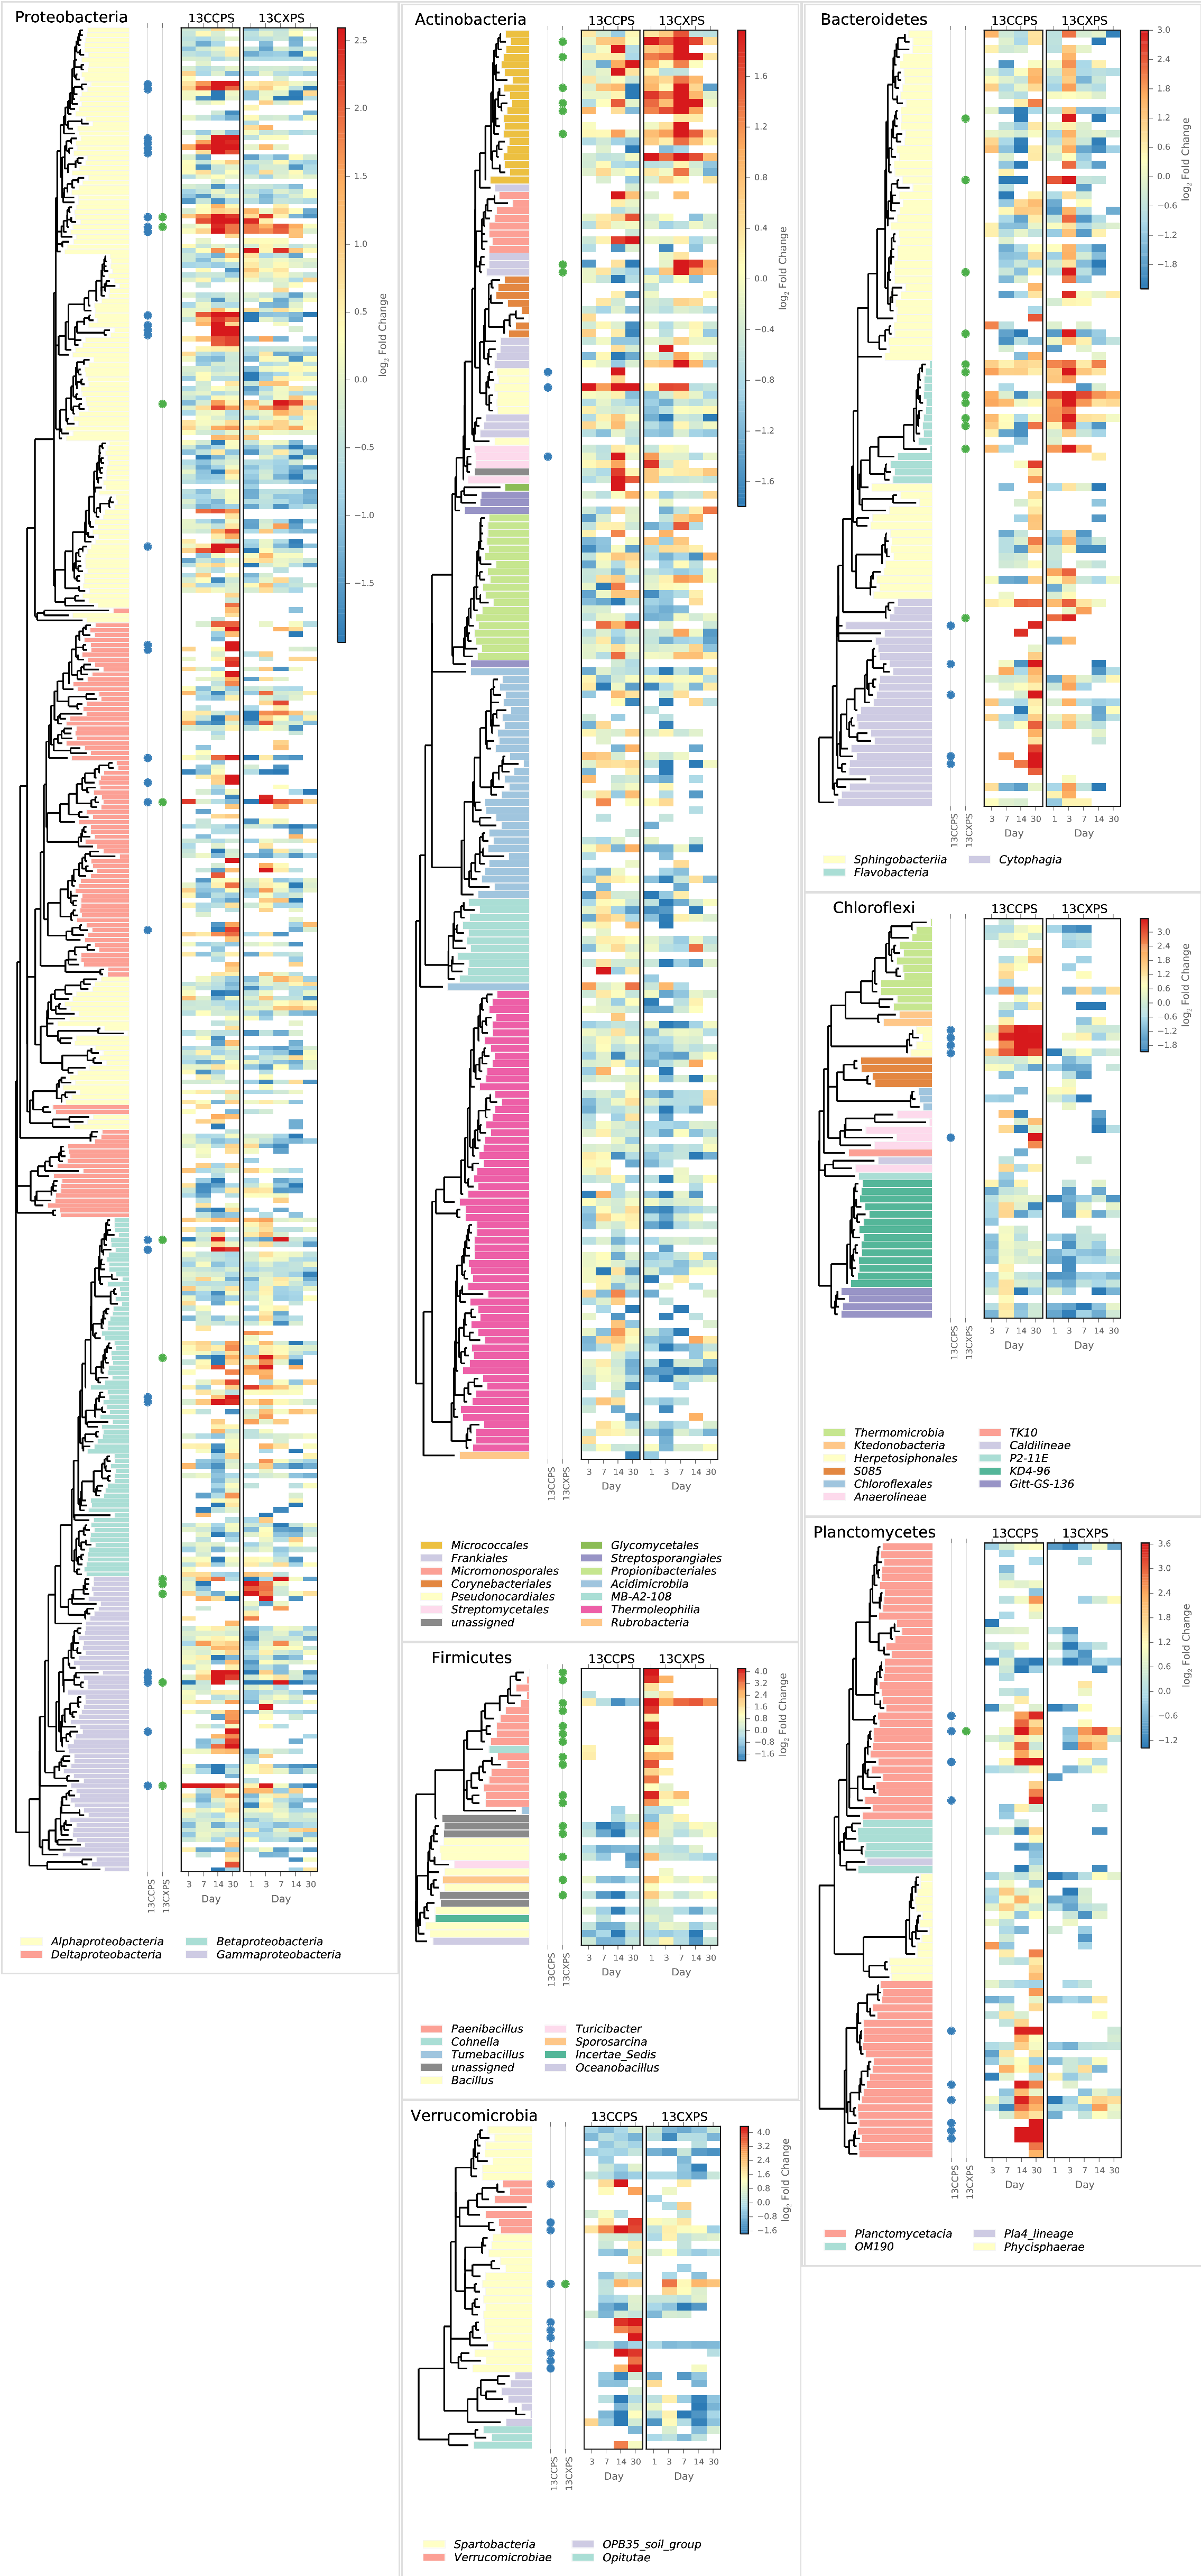
\includegraphics[width=0.65\textwidth]{figures/tiled_tree/tiled_tree.png}}
    \caption[Phylogenetic trees]{\protectPhylogenetic relationships of OTUs passing independent filtering when quantifying
OTU enrichment in heavy gradient fractions relative to control (see Methods). Only
those phyla that contain responders are shown. Colored dots are used to identify
xylose responders (green) and cellulse responders (blue). The heatmaps indicate
enrichment in high denstiy fractions relative to control (represented as LFC)
for each OTU in response to both $^{13}$C-cellulose (``13CCPS'', leftmost
heatmap) and $^{13}$C-xylose (``13CXPS'', rightmost heatmap) with values for
different days in each heatmap column. Greater enrichment (represented as LFC)
in heavy density fractions provide evidence of $^{13}$C-labeled DNA.

}\label{fig:tiledtree}
    \end{center} 
\end{figure*}

\begin{figure*}[H]
	\begin{center}
	\centerline{\includegraphics[width=0.6\textwidth]{figures/xylose_rspndr_bar/xylose_rspndr_bar.pdf}}
	\caption{\protectXylose reponders in the \textit{Actinobacteria}, \textit{Bacteroidetes},
\textit{Firmicutes} exhibit distinct temporal dynamics of $^{13}$C-labeling.
The left column shows counts of $^{13}$C-xylose responders in the
\textit{Actinobacteria, Bacteroidetes, Firmicutes} and \textit{Proteobacteria}
at days 1, 3, 7 and 30. The right panel shows enrichment in high density
gradient fractions (expressed as fold change, not logarithmic) for responders
(large points) as well as a boxplot for the distribution of fold change values
(small dots are outliers, i.e. beyond 1.5 times the interquartile range (IR).
Whiskers extend to 1.5 times the IR, and the box extends one IR about the
median (solid line)). Each day in the right column shows all responders (i.e.
OTUs that responded to xylose at any point in time). Greater enrichment in high
density fractions of $^{13}$C-xylose treatment relative to control indicates
DNA is $^{13}$C-labeled.
    
}\label{fig:xyl_count}
        \end{center}
\end{figure*}

\begin{figure*}[H]
	\begin{center}
	\centerline{\includegraphics[width=15.4cm]{figures/shift_and_rabund3/shift_and_rabund.png}}
	\caption{\protectCharacteristics of xylose responders (green) and cellulose responders (blue)
based on estimated \textit{rrn} copy number (A), $\Delta\hat{BD}$ (B), and
relative abundance in non-fractionated DNA (C). The estimated \textit{rrn} copy
number of all responders is shown versus time (A). Kernel density histogram of
$\Delta\hat{BD}$ values shows cellulose responders had higher average
$\Delta\hat{BD}$ than xylose responders indicating higher average atom \%
$^{13}$C in OTU DNA (B). The final panel indicates the rank relative abundance
of all OTUs observed in the non-fractionated DNA (C) where rank was determined
at day 1 (bold line) and relative abundance for each OTU is indicated for all
days by colored lines (see legend). Xylose responders (green ticks) have higher
relative abundance in non-fractionated DNA than cellulose responders (green ticks). 
All ticks are based on day 1 relative abundance.
}\label{fig:shift}
    \end{center}
\end{figure*}


\restoregeometry
